%% The following is a directive for TeXShop to indicate the main file
%%!TEX root = diss.tex

\chapter{Introduction}
\label{ch:Introduction}

This first paragraph will give a little intro and describe what is coming up in \autoref{sec:Cosmology}, \autoref{sec:Lensing} and \autoref{sec:Clusters}.

%%%%%%%%%%%%%%%%%%%%%%%%%%%%%%%%%%%%%%%%%%%%%%%%%%%%%%%%%%%%%%%%%%%%%%
\section{Cosmology}
\label{sec:Cosmology}

\subsection{Our Universe}

The \acf{CFHTLenS} was a big lensing project in the \acf{CFHTLS} survey. This is an example of an acronym that does not go in the table of acronyms:  \acs{UBC}. This section is supposed to be on cosmology...

\subsection{Distances in Cosmology}

%%%%%%%%%%%%%%%%%%%%%%%%%%%%%%%%%%%%%%%%%%%%%%%%%%%%%%%%%%%%%%%%%%%%%%
\section{Galaxy Clusters}
\label{sec:Clusters}

\subsection{Clusters as Cosmological Probes}

\subsection{Intracluster Physics}

%%%%%%%%%%%%%%%%%%%%%%%%%%%%%%%%%%%%%%%%%%%%%%%%%%%%%%%%%%%%%%%%%%%%%%
\section{Gravitational Lensing}
\label{sec:Lensing}

As light from distance objects in the universe makes the journey from its source to our telescopes, it is deflected and distorted by mass inhomogeneities along its path. In particular, large overdensities, such as galaxies and galaxy clusters, will cause light rays to be bent 

\begin{figure}
\begin{center}
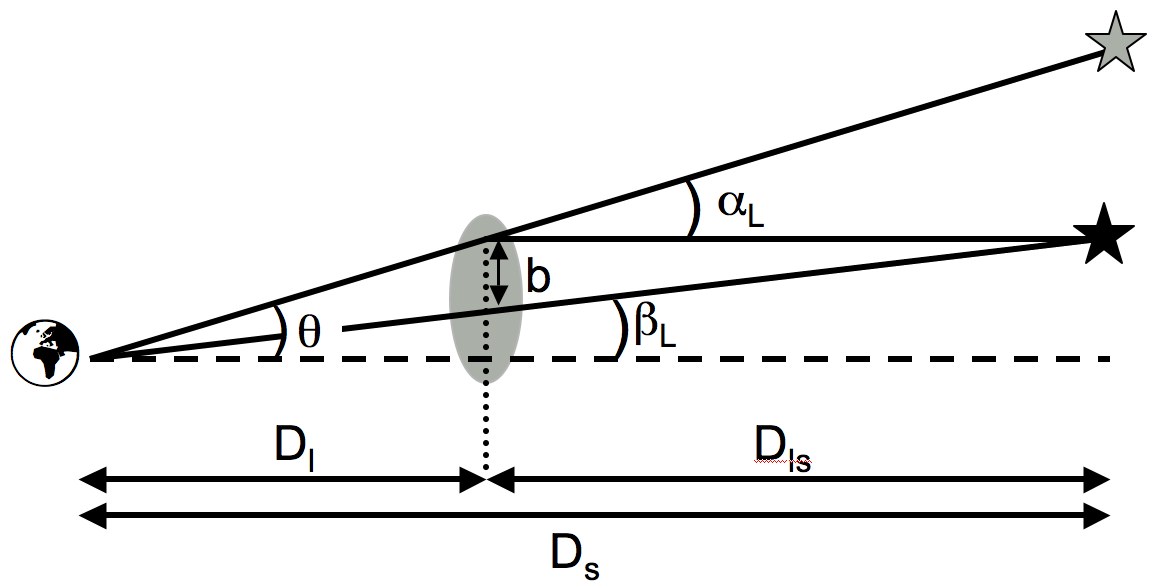
\includegraphics[scale=0.3]{plots_intro/LensDiagram.png}
\caption[Gravitational Lensing Diagram]{Diagram showing the geometry of gravitational lensing. Light from the background source is bent by an angle $\alpha$ when it passes near the gravitational lens (gray oval) on its way to the earth. While the actual source (black star) is at an angle $\beta$ relative to the horizontal, its image (gray star) appears to be at an angle $\alpha+\beta$. The angular diameter distances to the lens ($D_{\rm l}$), to the source ($D_{\rm s}$) and between the lens and source ($D_{\rm ls}$) are labeled.}
\label{lensing}
\end{center}
\end{figure}


\subsection{Weak Lensing Shear}

\subsection{Magnification}
\label{sec:mag}
Weak lensing magnification is, to first order, a measure of the convergence of a lensing mass.  It can be detected through the stretching of solid angle on the sky, which leads to the amplification of source flux, since lensing conserves surface brightness. In general, two different approaches can be taken to measure magnification.  The method we employ involves observing the effects on source number densities that result from source amplification in a flux-limited survey. An alternative approach is to observe coherent variations in source sizes and flux, but this method suffers from many of the limitations facing shear analysis.

Magnification affects the source number densities in two ways, and the one that dominates is determined by the intrinsic magnitude number counts of the sources in question.  Simply put, the brightest sources, which usually have steep number counts, will exhibit an {\it increase} in number density when lensed, as the amplification allows more objects to be detected, while the number density of the faintest sources, having relatively shallow number counts, will {\it decrease} \citep{Narayan89}.

Compared to shear measurements, magnification exhibits a slightly lower signal-to-noise ($S/N$) ratio, the reason it has been largely ignored until recently.  However, what magnification lacks in signal strength, it makes up for in terms of its ability to be applied to lenses at higher redshift and to poorly resolved sources \citep{Waerbeke10}.  Since shear studies require measurements of galaxy shapes, in order for a source to be used it must necessarily be well resolved.  This is in stark contrast to magnification studies using source number densities, which have no such requirement for the sources to be resolved at all.  In principle only source magnitudes, redshifts, and positions relative to a lens must be known.  This simple fact makes it possible to extend weak lensing magnification analyses to a much higher redshift than possible for shear, and allows a much higher source density to be included in the analysis.  

Because the constraint on source resolution is considerably relaxed, ground-based observations can be incorporated to a greater degree with magnification than for shear, as we are not concerned with correcting for the smearing of the image due to the Point Spread Function. From the financial perspective, magnification studies are therefore extremely cheap to carry out, since the excellent resolution of space-based telescopes is not required. See \citet{Waerbeke10}, \citet{RozoSchmidt10}, and \citet{Umetsu11}, for more detailed discussions of the benefits of combining magnification with shear in gravitational lensing studies.

The magnification factor $\mu$ is the inverse determinant of the amplification matrix, which maps the image deformation from the source to observer frame, and describes the first order effects of gravitational lensing \citep{BS01}.
\begin{equation}
\mu = \frac{1}{\mathrm{det} \cal{A}} = 
\frac{1}{(1-\kappa)^2 - \left|\gamma\right|^2} \approx 1+2\kappa
\label{mu}
\end{equation}
The magnification is simply a measure of the convergence ($\kappa$) of light rays due to the projected mass along the line-of-sight.  Assuming a model for a density profile, e.g. SIS or NFW, $\mu$ can then directly yield the surface-mass-density of the lens.

The number of observed source galaxies, as a function of magnitude and redshift, $n(m,z)$, is related to the intrinsic number $n_0(m,z)$ that would be observed in the absence of lensing through an equation involving properties of both the lens and source:
\begin{equation}
n(m,z)dm = \mu ^{\alpha -1} n_0(m,z)dm.
\end{equation}
where $\alpha$ is a property of the background sources, defined according to
\begin{equation}
\alpha \equiv \alpha(m,z) = 2.5 \frac{\mathrm d}{\mathrm d \it m} \log n_0(m,z).
\label{alpha}
\end{equation}
The form of this relationship was first demonstrated by \citet{Narayan89}, as it applied to lensed quasar number densities, but can be easily generalized to any galaxy type as long as one has a means of obtaining the slope of the number counts $\alpha$.

This shows that distant source galaxies, lensed by an intervening concentration of mass, may have their observed number counts increased {\it or} decreased depending on the sign of the quantity $\alpha -1$.  Sources for which $\alpha -1 > 0$ will appear to be correlated on the sky with a lens position, while sources with $\alpha -1 < 0$ will be anti-correlated, as a dearth of objects will be observed in the vicinity of a lens.  The number density of galaxies for which the intrinsic number count slope gives $\alpha -1 \approx 0$ will essentially be unaffected by lensing magnification, as the dilution and amplification effects will cancel, and no correlation signal will be observed for these objects \citep{Scranton05}.

The first measurement? or calculation? was by \citet{Broadhurst95}
Important early lensing calculations by \citet{KS93} First description of lensing for measuring mass was by \citet{Tyson84}. first realization that quasar excess around galaxies was due to lensing was by \citet{Narayan89}.

\subsection{Magnification vs. Shear}

%%%%%%%%%%%%%%%%%%%%%%%%%%%%%%%%%%%%%%%%%%%%%%%%%%%%%%%%%%%%%%%%%%%%%%
\section{Impact of this Thesis}
\label{sec:impact}

This work contained in this thesis has pushed the boundaries of what knowledge can be extracted from weak lensing surveys. By including intrinsically smaller and fainter background sources, which cannot be used in conventional weak lensing studies, we pave the way for a more optimal use of survey data. These gravitationally-lensed sources, which are too small for reliable shape or size measurements, can still be included in a lensing analysis by using the flux magnification formalism described in Section \ref{sec:mag}. The author of this thesis has proven the utility of measuring magnification, through several key publications which appear as chapters in this work, and carried out thorough studies of the systematic effects which provide limitations. 

Prior to this thesis research, weak lensing was dominated by the shear method. This was originally motivated by some early work showing that the signal-to-noise for shear was several times larger than for magnification \citep{Schneider00}. While it is true that, for a fixed sample of galaxies, there is less scatter in galaxy shapes than in galaxy positions, the latter is far easier to measure. This simple fact has motivated the research herein. As lensing studies push to higher redshift, and increasingly rely on blurry ground-based data, we have elevated confidence in our measurements of source positions over difficult shape determinations. 

When this thesis work began, only a handful of magnification studies had been completed. The first ground-breaking theoretical formulation of how number densities of sources could be used to measure masses of clusters was laid out in 1995 by \citet{Broadhurst95}, but it took another 20 years before the first convincing observational detection was made \citep{Scranton05}. Following this significant $8\sigma$ detection of galaxy-magnified quasars in the \acf{SDSS}, several studies followed, achieving magnification detections for lensing of normal galaxies \citep{Hildebrandt09b}, and of blue galaxies behind strong lensing clusters \citep{Umetsu11}. These studies all stopped short of deriving scientifically useful results from the magnification measurements -- they either represented proof-of-concept studies for a new technique, or they demonstrated consistency with a lensing interpretation of the signal.

The work in this thesis made major steps forward in the area of lensing magnification. The author performed the first-ever measurement of magnification by stacked galaxy groups in 2012 (See Chapter \ref{ch2}). This particular work was also the first time that shear and magnification mass estimates and signal-to-noise had been compared \citep{Ford12}. Following this influential work in the \acf{COSMOS} survey, the thesis author transitioned focus to the much larger astronomical survey known as the \acf{CFHTLenS}. 

Two important studies resulted from magnification analyses of the \ac{CFHTLenS} for this thesis (See Chapters \ref{ch3} and \ref{ch4}). First of all, the most significant magnification detection thus far (at $9.7\sigma$) was published in \citet{Ford14}. More importantly, however, that work moved beyond simple magnification-detection to actual science. The thesis author measured masses of stacked galaxy clusters binned as a function of different attributes (redshift and richness), and the dependence of a magnification signal on these parameters was seen for the first time. A mass-richness scaling relation was determined solely from the magnification results, which is a useful tool for making cosmological inferences from optical cluster surveys, as discussed in \ref{sec:Clusters}. 

This work contained the important inclusion of a means of accounting for one of the dominant systematic effects for magnification, the contamination of the background sources with low-redshift objects. The formalism was extended from earlier work by \citet{Hildebrandt13}, but allowing for different contamination fractions and models for the halo occupation distribution of the galaxy contaminants. This was the first time that galaxy cluster lenses could be used for magnification in a redshift range where there was known source contamination. Prior to this work, the redshift ranges of overlap had to be avoided because the physically-induced cross-correlations of lens and source objects overwhelmed, and could not be separated from, the magnification signal.

Arguably the most important magnification result in all the literature to date is contained in Chapter \ref{ch4} of this thesis. After the semi-blind magnification analysis of \citet{Ford14}, \citet{Ford15} followed suit with an identical treatment of the same cluster sample, but this time using the weak lensing shear approach. This study contained a detailed comparison between cluster masses measured with the two independent techniques, as a function of different cluster attributes, and contained valuable insights regarding systematic effects that are still important to resolve for magnification. Moving forward, this work frames the case for including magnification, and also pin-points some important issues that must be addressed in future work (see Chapter \ref{ch:conc}).

%%%%%%%%%%%%%%%%%%%%%%%%%%%%%%%%%%%%%%%%%%%%%%%%%%%%%%%%%%%%%%%%%%%%%%
\section{Thesis Overview}
\label{sec:overview}

The body of this thesis is composed of three published studies that develop the weak gravitational lensing magnification technique, particularly for the study of galaxy clusters, and compare with results using the complementary and much more ubiquitous weak lensing shear approach:
\begin{itemize}
\item Chapter \ref{ch2} contains the first magnification study of galaxy groups and first comparison with shear for stacked lens samples. The data are X-ray selected groups, and high-redshift Lyman-break galaxies in the ac{COSMOS} field.
\item Chapter \ref{ch3} represents the highest-significance magnification detection, and the first magnification study that could be binned as a function of cluster parameters. The data are optically-selected galaxy clusters and high-redshift Lyman-break galaxies in the ac{CFHTLenS} field.
\item Chapter \ref{ch4} is the follow-up shear analysis of the same cluster sample presented in the previous chapter, using the ac{CFHTLenS} shear catalog for background source shape measurements.
\end{itemize}
Finally, Chapter \ref{ch:conc} wraps up with conclusions on the topic of cluster studies using both magnification and shear, and briefly outlines future directions for progress within the field.

%%%%%%%%%%%%%%%%%%%%%%%%%%%%%%%%%%%%%%%%%%%%%%%%%%%%%%%%%%%%%%%%%%%%%%
\endinput
Any text after an \endinput is ignored.
You could put scraps here or things in progress.
